%%
%% Meta: Formelsammlung GESO BBW
%% 2023 fp @ bbw.ch
%%


%% Alle Kommandos und entsprechende...
%%
%% Diverse Flags, um die Version zu steuern.
%% Individuelle Flags pro Lehrperson sind in den VERSION_<Kuerzel>.txt-Files
%%


%%
%%  Mandant: Für wen wurde die Formelsammlung erstellt
%% Überschreiben mit "\renewcommand{\versionMANDANT}{XYZ}
%%
\newcommand{\versionMANDANT}

%%%%%%%%%%%%%%%%%%%%%%%%%%%%%%%%%%%%%%%%%%%%%%%%%%%%%%%
%%        L A Y O U T   O P T I O N E N
%%%%%%%%%%%%%%%%%%%%%%%%%%%%%%%%%%%%%%%%%%%%%%%%%%%%%%%

\newif\ifisSCHWARZETITEL%% Titel schwarz statt BBW Grün 
\newcommand\SCHWARZETITEL[1]{\ifisSCHWARZETITEL%%
#1%%
\fi}%% End New Command SCHWARZETITEL
\isSCHWARZETITELtrue%%


\newif\ifisFONTHELVETICA%% Font Helvetica statt Times
\newcommand\FONTHELVETICA[1]{\ifisFONTHELVETICA%%
#1%%
\fi}%% End New Command ifFONTHELVETICA
\isFONTHELVETICAtrue%%



%%%%%%%%%%%%%%%%%%%%%%%%%%%%%%%%%%%%%%%%%%%%%%%%%%%%%%%
%%    O P T I O N E N   V A R I A B L E N N A M E N
%%%%%%%%%%%%%%%%%%%%%%%%%%%%%%%%%%%%%%%%%%%%%%%%%%%%%%%


\newif\ifisFAKTORAQ%% Formal mit a * q^t
\newcommand\FAKTORAQ[1]{\ifisFAKTORAQ%%
#1%%
\fi}%% End command FAKTORAQ
\isFAKTORAQtrue%%

\newif\ifisFAKTORBA%% Formel mit b * a^t
\newcommand\FAKTORBA[1]{\ifisFAKTORBA%%
#1%%
\fi}%% End New Command FAKTORBA
\isFAKTORBAfalse%%

%% Für Rahmenlehrplan (RLP)
\newif\ifisRLP
\newcommand\RLP[1]{\ifisRLP%%
#1%%
\fi}%% End New Command RLP
\isRLPtrue%

%%%%%%%%%%%%%%%%%%%%%%%%%%%%%%%%%%%%%%%%%%%%%%%%%%%%%%%
%%    I n h a l t s  -  O P T I O N E N
%%%%%%%%%%%%%%%%%%%%%%%%%%%%%%%%%%%%%%%%%%%%%%%%%%%%%%%

%% Zeigt die Grafik "Skalentypen" bei Datenanalyse
\newif\ifisMITSKALENTYPEN%%
\newcommand\MITSKALENTYPEN[1]{\ifisMITSKALENTYPEN%%
#1%%
\fi}%% End New Command MITSKALENTYPEN
\isMITSKALENTYPENfalse%%

%% Zeigt bei Zahldarstellungen/Runden auch das Kapitel
%% «Mit Signifikanten Stellen Runden»
\newif\ifisMITSIGNIFIKANTENSTELLEN%%
\newcommand\MITSIGNIFIKANTENSTELLEN[1]{\ifisMITSIGNIFIKANTENSTELLEN%%
#1%%
\fi}%% End New Command MITSIGNIFIKANTENSTELLEN
\isMITSIGNIFIKANTENSTELLENfalse%%

%% Sollen ALLE drei Log-Gesetze gezeigt werden, dann TRUEN
%% Ansonsten werden nur die im Rahmenlehrplan geforderten
%% dargestellt
\newif\ifisALLELOGGESETZE%%
\newcommand\ALLELOGGESETZE[1]{\ifisALLELOGGESETZE%%
#1%%
\fi}%% End New Command ALLE LOG GESETZE
\isALLELOGGESETZEfalse%%

%%
%% DEfinition, was bei statistischen Variablen ROBUST sein soll.
%%
\newif\ifisROBUSTDEFINITION%%
\newcommand\ROBUSTDEFINITION[1]{\ifisROBUSTDEFINITION%%
#1%%
\fi}%% End New Command ROBUSTDEFINITION
\isROBUSTDEFINITIONtrue%%


%% ... Auswahlen
%%
%% Version Freimann Gressly Philipp (GRPH)

\newcommand{\versionGRPH}{}
\renewcommand{\versionMANDANT}{(fp@bbw.ch)}

\isRLPfalse%%
\isMITSKALENTYPENfalse%%
\isFAKTORAQfalse%%
\isFAKTORBAtrue%%
\isMITSIGNIFIKANTENSTELLENfalse%%
\isSCHWARZETITELfalse%%
\isROBUSTDEFINITIONfalse%%
\isFONTHELVETICAfalse%%



\newcommand{\versionsDatumFoSa}{2023-04-07}
\newcommand{\versionIdSubRev}{0.5.0}
\newcommand{\versionsnummerFoSa}{\versionsDatumFoSa{} \versionIdSubRev\,\,\versionMANDANT}

\input{bbwLayoutPage}

\newcommand{\geometrieErsteSeite}{}

\ifdefined\versionDEST%%
\renewcommand{\metaHeaderLine}{}
\renewcommand{\geometrieErsteSeite}{\newgeometry{left=3mm,right=3mm,top=2mm,bottom=4mm}}
\else
\renewcommand{\metaHeaderLine}{Formelsammlung --- gesundheitlich-soziale BM}%% END HEADERFOOTER
\renewcommand{\geometrieErsteSeite}{\newgeometry{left=7mm,right=7mm,top=22mm,bottom=15mm}}
\fi%% END version DEST

%%\fancyhf[LE,FLO,FRE,FRO]{}%% Überscrheibe Titel
%%\MITHEADERFOOTER{\fancyhf[LE,FLO,FR]{Seite \thepage{}}}%% Überscrheibe Titel
\newcommand{\headerUndFooterErsteSeite}{%%
\ifdefined\versionDEST%%
\thispagestyle{empty}%%
\else
\thispagestyle{fancy} \fancyhf[HC]{\metaHeaderLine} \fancyhf[HR]{\thepage{}} \fancyhf[FR]{}%%
\fi%% version DEST
}%% END newcommand "headerUndFooterJedeSeite

\newcommand{\headerUndFooterJedeSeite}{%%
\ifdefined\versionDEST%%
\thispagestyle{empty}%%
\else
\thispagestyle{fancy} \fancyhf[HLE]{} \fancyhf[HC]{} \fancyhf[HR]{\thepage{}} \fancyhf[FR]{}%%
\fi%% version DEST
}%% END newcommand "headerUndFooterJedeSeite


\newcommand{\forceCB}{\vfill\null\columnbreak\headerUndFooterJedeSeite{}}


%%%%%%%%%%%%%%%%%%%%%%%%%%%%%%%%%%%%%%%%%%%%%%%%%%%%%%%%%%%%%%%%%%


%% Hintergrundfarbe in tabular

\usepackage{makecell}

\renewcommand{\shortAuthor}{fp he @ bbw.ch [\versionsnummerFoSa{}]}

\renewcommand{\arbeitsblattTitel}{}%%{Formelsammlung --- gesundheitlich-soziale BM\TRAINER{ (V \versionIdSubRev)}}

%% Millimeterpapier (2.8mm) für Notizen \mmPap
\newcommand{\mmPap}[1]{\mmPapierZwei{#1}{8.4}}

%% Listen nicht einrücken:
\setlist[itemize]{leftmargin=*}

%%\definecolor{FarnFarbe}{HTML}{4F8F00}

%%\renewcommand{\arbeitsblattHeader}{}




%%%%%%%%%%%%%%%%%%%%%%%%%%%%%%%%%%%%%%%%%%%%%%%%%%%%%%%%%%%%%%%%%%%%%%%%%%%%%%%%%%%%%%%%%%%%%%%%%%%%%%%%%%%%%%

%% Titel schwarz, nicht bbw Grün
\SCHWARZETITEL{\definecolor{titelFarbe}{rgb}{0,0,0}}%%

%% Helvetica Font (statt Times)
\FONTHELVETICA{%%
\usepackage{helvet}
\renewcommand{\familydefault}{\sfdefault}%%
}%%

\begin{document}%%

\geometrieErsteSeite{}

\font\myfont=cmr11 at 40pt


\headerUndFooterErsteSeite{}
%%%%%%%%%%%%%%%%%%%%%%%%%%%%%%%%%%%%%%%%%%%%%%%%%%%%%%%%%%%%%%%%%%%%%%%%%%%%%%%%%%%%%%%%%%%%%%%%%%%%%%%%%%%%%%%

%%\arbeitsblattHeader{}

\arbeitsblattTitel{}%% Nur auf erster Seite.

\begin{multicols}{2}%%



\section*{Dezimalzahlen}
\subsection*{Runden}
Bsp.: Runden auf \textbf{\color{farnFarbe}vier}  Dezimalen.
Betrachte die nächste Ziffer und runde auf, falls diese
{\color{red}Ziffer} $\ge 5$. Bsp.:

$3.\mathbf{\color{farnFarbe}4729}\mathbf{\color{red}6}44 \approx 3.\mathbf{\color{farnFarbe}4730}$; \hfill{ }
$70.\mathbf{\color{farnFarbe}0031}\mathbf{\color{red}4}998\approx 70.\mathbf{\color{farnFarbe}0031}$

(Alle vier Dezimalen sind anzugeben.)

\MITSIGNIFIKANTENSTELLEN{\subsection*{Signifikante Stellen}
Führende Nullen zählen nicht, nachfolgende Nullen
zählen. Bsp. \textbf{\color{farnFarbe}vier} signifikante Stellen:

$$\mathbf{\color{farnFarbe}208.0} \textrm{ cm} = \mathbf{\color{farnFarbe}2.080} \textrm{ m} = 0.00\mathbf{\color{farnFarbe}2080} \textrm{ km}$$
}%% END MITSIGNIFIKANTENSTELLEN

\MITWISSENSCHAFTLICHERNOTATION{%%
\subsection*{Wissenschaftliche Notation}
Bei der wissenschaftlichen Notation steht vor dem
Dezimalpunkt immer \textbf{\color{blue}genau eine Ziffer $\ge$ 1}:

\begin{tabular}{lcccr}
Zahl    & & wissenschaftl. & & TR: \tiprobutton{EE} \\
$3400$  &=& $\mathbf{\color{blue}3}.4\cdot{}10^3$ &=& \textbf{\color{blue}3}.4E3\\
$0.004$ &=& $\mathbf{\color{blue}4}\cdot{}10^{-3}$ &=& \textbf{\color{blue}4}E-3
\end{tabular}
}%% END  Mit Wissenschaftlicher Notation

\hrulefill%%
%%%%%%%%%%%%%%%%%%%%%%%%%%%%%%%%%%%%%%%%%%%%%%%%%%%%%%%%
%%               Algebra                              %%
%%%%%%%%%%%%%%%%%%%%%%%%%%%%%%%%%%%%%%%%%%%%%%%%%%%%%%%%
%%
\section*{Algebra}
\subsection*{Hierarchie der Operationen}
(1.) Klammern, (2.) Wurzeln/Potenzen,\\
(3.) Punktoperationen, (4.) Strichoperationen

\textbf{Termarten}

\begin{tabular}{rlrl}
$a+3x$  &Summe  & $5b^2-b$ & Differenz\\
$x(3-a)$&Produkt& $7:(b+1)$& Quotient\\
$(3x)^4$&Potenz &          &
\end{tabular}

\textbf{Achtung}

Differenzterm:  $3-(-7) = +10$

Produktterm:\, $-3(-7) = +21$

Produkt mit Produkt: $2\cdot(x\cdot{}y) = 2(xy) = 2xy$

Produkt mit Summe: $2\cdot(x+y)=2x+2y$

Potenzterme: $(-3)^2 = 9$ aber $-3^2 = -9$


Vorzeichen im Taschenrechner:\\
\vspace{3mm}\\
\tiprobutton{7}\tiprobutton{minus}\tiprobutton{2}$=7-2= 5$\\
\tiprobutton{7}\tiprobutton{neg}\tiprobutton{2}$=7(-2)=7\cdot{}(-2)= -14$

\subsection*{Binomische Formeln}
\begin{tabular}{lcl}
  $a^2 + 2ab + b^2$  & =  &  $(a+b)^2$\\
  $a^2 - 2ab + b^2$  & =  &  $(a-b)^2$\\
  $a^2 - b^2$        & =  &  $(a+b)(a-b)$
\end{tabular} 


\subsection*{(Absolut)betrag einer Zahl}%%
%%
\hfill\, $|+7| = 7$ \hfill\, $|-7| = 7$ \hfill\, %%

Geometrisch: Abstand zum Nullpunkt.

%%\RLP{\forceCB{}}
%%\hrulefill

\section*{Bruchterme}
    $\frac{a}b = a : b$,\phantom{ and }  $\frac{a}b : \frac{x}y = \frac{a}b\cdot{}\frac{y}x = \frac{ay}{bx}$
    
\subsection*{Faktorisieren (Beispiele)}

\begin{enumerate}
\item gemeinsame Faktoren ausklammern:
\begin{itemize}
\item Zahlen und Variable ausklammern
$$ax + ay = a(x+y)$$
\item
Teilsummen ausklammern
$$3(7r+6) - b(7r+6) = (3-b)(7r+6)$$
\begin{tabular}{rcl}
$ac+bc+ad+bd$ &=& $(a+b)c+(a+b)d$ \\
              &=& $(a+b)(c+d)$
\end{tabular}              

\item $(-1)$ ausklammern
  $$(b-a)=(-1)\cdot{}(a-b)$$
  $$(b-a)^2 = \left((-1)\cdot{}(a-b)\right)^2 = (a-b)^2$$
\end{itemize}

\item Binomische Formeln anwenden:
$$x^2-1 = (x-1)(x+1)$$
$$4b^2 -12bc + 9c^2=(2b-3c)^2$$
\item Zweiklammeransatz bilden:
$$x^2+2x-15 = (x+5)(x-3)$$

\end{enumerate}
%%%\forceCB{}%%


\subsection*{Summenzeichen}

  $${\color{farnFarbe}\sum_{{\color{red}k}{{\color{farnFarbe}{\color{black}=}\color{blue}1}}}^{\color{blue}n\color{farnFarbe}}}
  {\color{orange}T(}{{\color{red}k}}{\color{orange})} = {\color{orange}T(}{\color{blue}1}{\color{orange})} {\color{farnFarbe}+} {\color{orange}T(}{\color{blue}2}{\color{orange})} {\color{farnFarbe}+}
  ... {\color{farnFarbe}+} {\color{orange}T(}{\color{blue}n}{\color{orange})}$$

Beispiel

  $${\color{farnFarbe}\sum_{{\color{red}x}{{\color{farnFarbe}{\color{black}=}\color{blue}3}}}^{\color{blue}5\color{farnFarbe}}}  {\color{red}x}^{{\color{orange}7}} = {\color{blue}3}^{\color{orange}7} {\color{farnFarbe}+} {\color{blue}4}^{\color{orange}7} {\color{farnFarbe}+} {\color{blue}5}^{\color{orange}7}$$

\TRAINER{TR nur am Schluss?}
%%Taschenrechner (\texttt{sum}): \tiprobutton{math}\tiprobutton{5}


%% Forced column break
%%\forceCB

\hrulefill
%%%%%%%%%%%%%%%%%%%%%%%%%%%%%%%%%%%%%%%%%%%%%%%%%%%%%%%%
%%               Potenzen                             %%
%%%%%%%%%%%%%%%%%%%%%%%%%%%%%%%%%%%%%%%%%%%%%%%%%%%%%%%%
\section*{Potenzen}
\begin{tcolorbox}[colback=white]
\bbwCenterGraphic{5cm}{img/Potenzbegriff.png}
$$a^n = \underbrace{a\cdot{}a\cdot{}a\cdot{}...\cdot{}a}_{n\textrm{ Faktoren}}$$
Für $a\ne 0$ gilt:
$$a^{-n} = \frac1{a^n}$$
  $$a^0 = 1$$
\end{tcolorbox}

\subsection*{gleiche Basis}
$a^m\cdot{}a^n = a^{m+n}$ \hspace{2cm} $a^m:a^n=a^{m-n}$


\subsection*{Potenzieren einer Potenz}
$\left(a^m\right)^n = a^{m\cdot{}n}$ 

\subsection*{gleicher\,Exponent}
\begin{tabular}{cc}
$a^n\cdot{}b^n = (a\cdot{}b)^n,$ & $\frac{a^n}{b^n} =\left(\frac{a}b\right)^n $
 \end{tabular}

\subsection*{Vorzeichen}
Fall: $n$ \textbf{gerade}:

\begin{tabular}{cc}
 $-(a^n) = -a^n,$ & aber: $(-a)^n = +a^n$
 \end{tabular} 

Fall: $n$ \textbf{un}gerade:

\begin{tabular}{cc}
 $-(a^n) = -a^n,$ & aber: $(-a)^n = -a^n$
 \end{tabular} 


\subsection*{negative Exponenten}

%%Für Basis $a\ne 0, b\ne 0$ und $m \in\mathbb{Q}$ gilt:

\begin{tabular}{cc}
$a^{-m} = \frac1{a^m},$ & $\left(\frac{a}b\right)^{-m} = \left(\frac{b}a\right)^m$
 \end{tabular}

Exponenten vertauschen ihr Vorzeichen beim Übertreten des
Bruchstrichs. Beispiel:
$$\frac{a^{-3}b^2}{c^5d^{-6}} = \frac{b^2d^6}{a^3c^5}$$

%%\forceCB{}

\subsection*{$n$-te Wurzel}
$\sqrt[n]{a} = \left(a\right)^\frac1n$\hfill{}Bsp.: $8^{\frac13}=\sqrt[3]{8}=2$

\begin{tcolorbox}[colback=white]
$$a^{\frac{m}n} = \sqrt[n]{a^m} = \left(\sqrt[n]a\right)^m$$
$$\sqrt[n]{\sqrt[m]{a}}   = \left((a)^\frac1m \right)^\frac1n =
  a^\frac1{nm} = \sqrt[m]{\sqrt[n]{a}}   = \sqrt[mn]{a}$$

  $$\sqrt[n]{a\cdot{}b} = \sqrt[n]{\vphantom{b}a} \cdot \sqrt[n]b$$

  $$\sqrt[n]{\frac{a}{b}} = \frac{\sqrt[n]a}{\sqrt[n]b}$$
\end{tcolorbox}

%%$$\sqrt[n]{a\cdot{}\sqrt[m]b} =   \sqrt[n]{\vphantom{b}a} \cdot \sqrt[n m]b$$
%%
 
%%\forceCB%%
\hrulefill
%%%%%%%%%%%%%%%%%%%%%%%%%%%%%%%%%%%%%%%%%%%%%%%%%%%%%%%%
%%               Logarithmen                          %%
%%%%%%%%%%%%%%%%%%%%%%%%%%%%%%%%%%%%%%%%%%%%%%%%%%%%%%%%
\section*{Logarithmen}
\headerUndFooterJedeSeite{}

\begin{tcolorbox}[colback=white]
  \textbf{Definition Logarithmus}\\
  Für $b>0, b\ne 1, a>0$ ist

$$\log_b{}(a)=x \Longleftrightarrow{} b^x = a$$
\end{tcolorbox}

Logarithmen sind Exponenten zu einer fest gewählten Basis. Häufige Basen:

$$\lg = \log_{10} $$
$$\ln = \log_e$$
$$e \approx 2.71828 \textrm{ = Eulersche Konstante}$$


\begin{tcolorbox}[colback=white]
\ALLELOGGESETZE{$$\log(u\cdot v) = \log(u) + \log(v)$$}
\ALLELOGGESETZE{$$\log(u : v) = \log(u) - \log(v)$$}

\FAKTORBA{$$\log(b^x) = x\cdot{}\log(b)$$
$$\log_{\color{farnFarbe}a}({\color{red}b}) = \frac{\lg({\color{red}b})}{\lg({\color{farnFarbe}a})} = \frac{\ln({\color{red}b})}{\ln({\color{farnFarbe}a})}$$}
\FAKTORAQ{$$\log(a^x) = x\cdot{}\log(a)$$
$$\log_{\color{farnFarbe}b}({\color{red}a}) = \frac{\lg({\color{red}a})}{\lg({\color{farnFarbe}b})} = \frac{\ln({\color{red}a})}{\ln({\color{farnFarbe}b})}$$}
\end{tcolorbox}%
%
%%\RLP{\forceCB{}}%%
%%\forceCB{}%%

%%%%%%%%%%%%%%%%%%%%%%%%%%%%%%%%%%%%%%%%%%%%%%%%%%%%%%%%
%%               Gleichungen                          %%
%%%%%%%%%%%%%%%%%%%%%%%%%%%%%%%%%%%%%%%%%%%%%%%%%%%%%%%%
\section*{Gleichungen}
                
\subsection*{Lineare Gleichungen}
Grundform: $ax+b=0$

Beispiel mit Parametern:
$$a^2x-b=b^2x+a$$
$$x\textrm{ auf eine Seite\, } \Longrightarrow a^2x -b^2x = a+b$$
$$x\textrm{ ausklammern }\Longrightarrow (a^2-b^2)x= a+b$$
$$\Longrightarrow x= \frac{a+b}{a^2-b^2} = \frac{a+b}{(a-b)(a+b)}=\frac{1}{a-b}$$

\subsection*{Quadratische Gleichungen}

\textbf{Grundform}: $ax^2 + bx+c = 0$

\begin{tcolorbox}[colback=white]
  \textbf{Lösungsformel}
  $$x_{1,2} = \frac{-b \pm \sqrt{b^2-4ac}}{2a}$$
\end{tcolorbox}
\textbf{Diskriminante} $D = b^2-4ac$\\
$D>0\Longrightarrow$ Zwei Lösungen;\\
$D=0\Longrightarrow$ Eine Lösung;\\
$D<0\Longrightarrow$ Keine Lösung

\subsubsection*{Spezialfälle}
\begin{itemize}
\item Lösen durch Faktorisieren:\\
$x^2+2x-15=0 \Longrightarrow (x-3)(x+5)=0 \Longrightarrow \lx=\{-5; 3\}$ %% DMK: (-5, 3) statt ;

\item Lösen durch Substitution:\\
$x^4+2x^2-15=0 \stackrel{y=x^2}{\Longrightarrow}\\
y^2+2y-15=0 \Longrightarrow \LoesungsMenge{}_y=\{-5;3\} \stackrel{x=\pm{}\sqrt{y}}{\Longrightarrow}
\textrm{ (Rücksubstitution) } \lx=\{\pm\sqrt{3}\}\\
\textrm{(} \pm\sqrt{-5} \textrm{ \, sind keine reelen Lösungen. )}$

\end{itemize}

\subsection*{Bruchgleichungen}

\textbf{Definitionsbereich} $\mathcal{D}$: Welche Werte dürfen in die Terme eingesetzt werden?

Bsp.: Nenner darf nicht Null werden:

$$\frac5{x+2}=\frac{7+x}{x-3} \Rightarrow{} \mathcal{D}_x=\mathbb{R}\backslash{}\{-2; 3\}$$

\subsection*{Potenzgleichungen}

%%  \TRAINER{ev. nur letztes Gesetz: $x^a = c$ und $x^\frac1b =c$ sind darin enthalten.  }

\begin{tabular}{lcl}
$k$ gerade:   $x^k=c$ & $\Leftrightarrow$ & $x=\pm\sqrt[k]{c}$\\
$k$ ungerade: $x^k=c$ & $\Leftrightarrow$ & $x=\sqrt[k]{c}$\\
%%$x^\frac1b=c$&$\Leftrightarrow$&$x=c^b$\\
%%$x^{\frac{a}b} = c$&$\Leftrightarrow{}$&$x=c^{\frac{b}a}
%%= \sqrt[a]{c^b}$
\end{tabular}

Beispiele

\begin{tabular}{rcl}
$x^4=16$ & $\Longrightarrow$ & $\lx=\{-2; 2\}  $ \\
$x^5=32$ & $\Longrightarrow$ & $\lx=\{+2\}  $ \\

\end{tabular}

\subsection*{Exponentialgleichungen}
\subsubsection*{mit Exponentenvergleich}

$$5^4 = 5^{2x+1} \Longrightarrow  4=2x+1$$

\subsubsection*{durch Logarithmieren}
\FAKTORBA{$$a^x=b \Rightarrow{} x=\log_a(b) = \frac{\lg(b)}{\lg(a)}$$}
\FAKTORAQ{$$b^x=a \Rightarrow{} x=\log_b(a) = \frac{\lg(a)}{\lg(b)}$$}


\subsection*{Lineare Gleichungssysteme}
\textbf{Grundform}:
\gleichungZZ{5x+7y}{19}{6x -3y}{57}

\begin{itemize}
\item Additionsverfahren
\item Einsetzungsverfahren
\item Gleichsetzungsverfahren
\item Graphisch oder \textbf{Taschenrechner}
\end{itemize}
Die Lösung ist ein geordnetes Zahlenpaar:
$$\LoesungsMenge{}_{(x | y)} = \{(8 | -3)\}$$


%%\forceCB

\headerUndFooterJedeSeite{}

\subsection*{Substitution}
Beispiel Bruchgleichungssysteme:

\gleichungZZ{{\color{farnFarbe}\frac6{x+1}} + {\color{red}\frac8{y-2}}}{11}{{\color{farnFarbe}\frac2{x+1}} - {\color{red}\frac{10}{y-2}}}{-9}
Substituiere
${\color{farnFarbe}a}={\color{farnFarbe}\frac1{x+1}}$ und
${\color{red}b} = {\color{red}\frac1{y-2}}$:

\gleichungZZ{{6\color{farnFarbe}a} + 8{\color{red}b}}{11}{2{\color{farnFarbe}a} - 10{\color{red}b}}{-9}

$$a=\frac12, b=1$$
Dann: Rücksubstitution
$$a=\frac12=\frac{1}{x+1} \Longrightarrow  x=1$$
$$b=1=\frac{1}{y-2} \Longrightarrow  y=3$$


%%\forceCB
%%\headerUndFooterJedeSeite{}

%%%%%%%%%%%%%%%%%%%%%%%%%%%%%%%%%%%%%%%%%%%%%%%%%%%%%%%%
%%               Textaufgaben                         %%
%%%%%%%%%%%%%%%%%%%%%%%%%%%%%%%%%%%%%%%%%%%%%%%%%%%%%%%%
\section*{Textaufgaben}
\subsection*{Geschwindigkeitsaufgaben}
\fbox{$s = v\cdot{} t$} (Einheiten kompatibel wählen!)\\
$s$ = Strecke; $v$ = Geschwindigkeit; $t$ = Zeit

\subsection*{Leistungsaufgaben}
Bei $x$ Zeiteinheiten für die ganze Arbeit:

Leistung = Arbeit pro Zeiteinheit

Leistung = $\frac{1 \textrm{ [Arbeit]}}{x \textrm{ [Zeiteinheiten]}}$

%%hysik: Leistung = $\frac{\textrm{[Joule]}}{\textrm{[Sekunde]}} = [\textrm{Watt}]$ \TRAINER{Watt ev weglassen?}

\subsection*{Restaufgaben}
$$A:B = C \textrm{ Rest } R \Leftrightarrow{}\frac{A-R}B=C$$


\subsection*{Zinseszins}
\begin{itemize}
\item $K_0$ = Startkapital; $K_n$ = Endkapital
\item $p$ = Zinssatz (in \%);\\ $a = 1+\frac{p}{100}$ = Zinsfaktor
(Wachstumsfaktor);\\ $p<0$, so ist $a$ der Zerfallsfaktor
\end{itemize}
$$K_n = K_0 \cdot{} \left( 1+\frac{p}{100} \right)^n = K_0\cdot{}a^n$$

Beispiele:
$$p = 2.5\% \Longleftrightarrow{} a = 1.025$$
$$p = -3\% \Longleftrightarrow{}  a = 0.97 $$


%%\forceCB

\headerUndFooterJedeSeite{}

%%%%%%%%%%%%%%%%%%%%%%%%%%%%%%%%%%%%%%%%%%%%%%%%%%%%%%%%
%%               Funktionen                           %%
%%%%%%%%%%%%%%%%%%%%%%%%%%%%%%%%%%%%%%%%%%%%%%%%%%%%%%%%
\section*{Funktionen}
\headerUndFooterJedeSeite{}


Eine Funktion ist eine {\color{red} eindeutige Zuordnung}. Dabei wird
jedem {\color{farnFarbe}x} aus der {\color{farnFarbe}Definitionsmenge
$\mathcal{D}$} eindeutig ein {\color{blue}y} aus der
{\color{blue}Wertemenge $\mathcal{W}$} zugeordnet. Beispiel:

\bbwCenterGraphic{8cm}{FunktionDefinition.pdf}


\ifdefined\versionDEST%
\else%%
\forceCB{}%%
\fi%%

\subsection*{Lineare Funktionen}

$$f\-:\,\,\,\,\, y = f(x) = a\cdot{}x + b \RLP{\textrm{\,\,\,\,oder\,\,\,\,} f(x)=m\cdot{}x + q}$$


\bbwCenterGraphic{8cm}{img/FunktionenLineareEinfuehrungHECH.pdf}

Steigung:

\fbox{$a$$ = \frac{\Delta y}{\Delta x} = \frac{y_2-y_1}{x_2-x_1}$}\\

Zwei Geraden sind \textbf{parallel}, wenn ihre Steigungen gleich sind.

$b$ = $y$-Achsenabschnitt (=Ordinatenabschnitt)

%%\forceCB

\headerUndFooterJedeSeite{}

\subsubsection*{Horizontale Gerade}

$g\-:\,\,\, y=ax+b$ ist horizontal, wenn die Steigung $a$ Null ist.

$$g\-:\,\,\,  y=0\cdot{}x+b \Rightarrow y=b$$


\ifdefined\versionHECH%%
\subsubsection*{Punkt- / Steigungsform}
Gerade durch Punkt $P=(P_x|P_y)$ mit gegebener Steigung $a$:
$$y = a(x-P_x) + P_y$$
\fi

\subsection*{Achsenschnittpunkte}

\textbf{Nullstelle}: Schnittstelle mit der $x$-Achse:\\
$y=0$ setzen und $x$ ausrechnen.


\textbf{Schnittpunkt mit der $y$-Achse}:\\
$x=0$ setzen und $y$ ausrechnen.


\subsection*{Schnittpunkt zweier Geraden}
Gegeben: $g\-:\,\,\, y=ax+b$ und $h\-:\,\,\, y=cx+d$.

Gleichsetzen: $ax+b = cx+d$ und nach $x$ auflösen.
%%\vspace{2cm}

%%\subsection*{Mittelpunkt $M$ einer Strecke $\overline{AB}$}
%%Gegeben: $A=(x_A|y_A)$ und $B=(x_B|y_B)$

%%Gesucht: Mittelpunkt $M=(x_M|y_M)$

%%Lösung Mittelwert $x$ und $y$ separat:

%%$$x_M = \frac{x_A+x_B}2; y_M=\frac{y_A+y_B}2$$

%%\headerUndFooterJedeSeite{}

\subsection*{Zweipunkte Aufgaben}


Gesucht Gerade $g\-: \,\,\, y=ax+b$ durch zwei gegebene Punkte $A=(x_A|y_A)$ und $B=(x_B|y_B)$


\textbf{Variante 1}: Steigung $a$ berechnen und einen der beiden Punkte in
$y=ax+b$ einsetzen, um $b$ zu finden.


\textbf{Variante 2}: Gleichungssystem nach $a$ und $b$ auf\/lösen:
\gleichungZZ{y_A}{a\cdot{}x_A+b}{y_B}{a\cdot{}x_B + b}

\textbf{Variante 3}: Punkte in \texttt{L1}=$x$ und \texttt{L2}=$y$
unter \tiprobutton{data} eingeben. Danach unter
\tiprobutton{2nd}\tiprobutton{data_stat-reg-distr} die «4» wählen:
\texttt{LinReg ax+b}.

\end{multicols}

%%%%%%%%%%%%%%%%%%%%%%%%%%%%%%%%%%%%%%%%%%%%%%%%%%%%%%%%%%%%%%%%%%%%%%%%%%%%%%%%%%%%%%%%%%%%%%%%%%%%%%%%%%%%%%%%%%
\newpage
\headerUndFooterJedeSeite{}

\subsection*{Potenzfunktionen}

\begin{tabular}{cc}
$k$ > 0: Parabel ($k$ gerade) & $k$ > 0: Parabel ($k$ ungerade)\\   %%\bbwCenterGraphic{8cm}{PotenzFkt.pdf}
  \includegraphics[width=73mm]{PotenzFktx2x4.pdf} &
  \includegraphics[width=73mm]{PotenzFktx3x5.pdf}\\

$k<0$: Hyperbel  ($k$ gerade) & $k<0$: Hyperbel ($k$ ungerade)\\
  \includegraphics[width=73mm]{PotenzFkt1overx2x4.pdf}&
  \includegraphics[width=73mm]{PotenzFkt1overx3x5.pdf}
  \end{tabular}


\begin{multicols}2

\begin{tcolorbox}[colback=white]
  \textbf{Grundform der Potenzfunktion}
$$y=ax^k$$
$k \in \{...-2, -1, 2, 3, 4, ...\}$
\end{tcolorbox}

$k$ gerade: Achsensymmetrisch ($y$-Achse)

$k$ ungerade: Punktsymmetrisch (Ursprung $O=(0|0)$)

%%Ist ${\color{green}a>0}$, so sind Graphen mit
%%geraden Exponenten nach oben geöffnet bzw. mit ungeraden Exponenten im
%%Quadranten I und III.

%%Ist ${\color{blue}a<0}$, so werden Graphen der obigen Funktionen an der $x$-Achse gespiegelt.

%% \includegraphics[width=4cm]{allg/funktionen/img/potenzfct/potenzFunktionenGerade.png}\hfill{}\includegraphics[width=4cm]{allg/funktionen/img/potenzfct/potenzFunktionenUngerade.png}
  \subsection*{Streckung / Spiegelung}
  Der Faktor $a$ in $y=a\cdot{}x^k$ streckt die Funktion in
  $y$-Richtung, bzw. spiegelt die Funktion an der $x$-Achse, wenn
  $a<0$ ist.
  \bbwCenterGraphic{73mm}{PotenzFktTransformation.pdf}



%%\hrulefill  
\forceCB
%%\headerUndFooterJedeSeite{}

%%%%%%%%%%%%%%%%%%%%%%%%%%%%%%%%%%%%%%%%%%%%%%%%%%%%%%%%
%%               Wachstumsmodelle                     %%
%%%%%%%%%%%%%%%%%%%%%%%%%%%%%%%%%%%%%%%%%%%%%%%%%%%%%%%%
\section*{Wachstumsmodelle}

\textbf{Lineares Wachstum}
$$f(t) = \FAKTORBA{a}\FAKTORAQ{m}\cdot t + \FAKTORBA{b}\FAKTORAQ{q}$$
Bei linearem Wachstum wird pro Zeiteinheit der selbe Wert $\FAKTORBA{a}\FAKTORAQ{m}$ \textbf{addiert}.

\textbf{Exponentielles Wachstum}

\FAKTORBA{$$f(t) = b\cdot{}a^t$$}
\FAKTORAQ{$$f(t) = a\cdot{}q^t$$}
Bei exponentiellem Wachstum wird pro Zeiteinheit mit dem selben Wert $\FAKTORBA{a}\FAKTORAQ{q}$ \textbf{multipliziert}.

  \begin{tabular}{rl}
   $\FAKTORBA{b}\FAKTORAQ{a}$  & Startwert bei $t=0$; $\FAKTORBA{b}\FAKTORAQ{a}=f(0)$\\
        & \phantom{$b$} = $y$-Achsenabschnitt\\
   $\FAKTORBA{a}\FAKTORAQ{q}$  & beschreibt das Wachstum
  \end{tabular}

$$A_0 = A(0) = f(0); A_t = A(t) = f(t)$$

\FAKTORBA{\bbwCenterGraphic{8cm}{ExpFktVergleichMitLinearemWachstumHECH.pdf}}
\FAKTORAQ{\bbwCenterGraphic{8cm}{ExpFktVergleichMitLinearemWachstumRLP.pdf}}

\subsection*{Exponentialfunktionen}
%%\bbwCenterGraphic{8.5cm}{allg/funktionen/img/exp/exponentielles_wachstum.png}
\begin{tcolorbox}[colback=white]$$y=f(t) = \FAKTORBA{b}\FAKTORAQ{a}\cdot{}{\FAKTORBA{a}\FAKTORAQ{q}}^t$$\end{tcolorbox}

Wachstum:
\FAKTORBA{$a>1$, Zerfall: $0<a<1$}
\FAKTORAQ{$q>1$, Zerfall: $0<q<1$}


\begin{tcolorbox}[colback=white]
Wachstum bezogen auf eine Zeitspanne  
  $$f(t) = {\color{blue}\FAKTORBA{b}\FAKTORAQ{a}}\cdot{}{\color{red}\FAKTORBA{a}\FAKTORAQ{q}}^{\frac{t}{\color{farnFarbe}\tau}}$$
  \begin{tabular}{ccp{60mm}}
$\color{farnFarbe}\tau$ &=& Beobachtungsintervall zu $\color{red}\FAKTORBA{a}\FAKTORAQ{q}$\\
    $\color{red}\FAKTORBA{a}\FAKTORAQ{q}$ &=& Wachstums(bzw. Zerfalls)rate im Zeit\-raum $\color{farnFarbe}\tau$
    \end{tabular}

Beispiel: Die Algen mit Startwert von ${\color{blue}3} \textrm{ m}^2$ ver{\color{red}vier}fachen
sich alle {\color{farnFarbe}fünf} Tage:\\
${\color{blue}\FAKTORBA{b}\FAKTORAQ{a}}={\color{blue}3}$, ${\color{red}\FAKTORBA{a}\FAKTORAQ{q}}={\color{red}4}$, ${\color{farnFarbe}\tau}={\color{farnFarbe}5}$
$$f(t)= {\color{blue}3}\cdot{}{\color{red}4}^\frac{t}{\color{farnFarbe}5}$$
\end{tcolorbox}
\FAKTORAQ{\bbwCenterGraphic{8cm}{ExponentialfctAQ.png}}
\FAKTORBA{\bbwCenterGraphic{8cm}{ExponentialfctAB.png}}

\subsection*{Basis $e$, Zeitvariable $x$}
$e$ = Eulersche Konstante $\approx 2.71828$
\FAKTORBA{$$y=b\cdot{}a^x$$ entspricht
$$y=b\cdot{}e^{mx}$$}

\FAKTORAQ{$$y=a\cdot{}q^x$$ entspricht
$$y=a\cdot{}e^{bx}$$}

\FAKTORBA{$\textrm{mit } a = e^m \,\,\textrm{ oder }  m = \ln(a)$}%
\FAKTORAQ{$\textrm{mit }  q = e^b \,\,\textrm{ oder }  b = \ln(q)$}%

\vspace{2mm}

\hrulefill

Und mit Zeitintervall $\tau$:

\FAKTORBA{$$y=b\cdot{}a^\frac{x}\tau$$ entspricht
$$y=b\cdot{}e^{mx}$$}
\FAKTORAQ{$$y=a\cdot{}q^\frac{x}\tau$$ entspricht
$$y=a\cdot{}e^{bx}$$}

\FAKTORBA{$\textrm{mit } a = e^{m\tau}  \,\,\textrm{ oder }    m=\ln\left(a^\frac1\tau\right) = \frac1\tau \cdot{}\ln(a)$}
\FAKTORAQ{$\textrm{mit }  q = e^{b\tau}  \,\,\textrm{ oder }    b=\ln\left(q^\frac1\tau\right) = \frac1\tau \cdot{}\ln(q)$}

\hrulefill
\subsection*{Halbwertszeit}
\ifisHALBWERTSZEITMITTAU%%
\FAKTORBA{$\frac12 \cdot{} b = f(t) = b\cdot{}a^{\frac{t}{\tau}}\phantom{xxx}\Longrightarrow\phantom{xxx}t= \tau\cdot{}\log_a\left(\frac12\right)$}
\FAKTORAQ{$\frac12 \cdot{} a = f(t) = a\cdot{}q^{\frac{t}{\tau}}\phantom{xxx}\Longrightarrow\phantom{xxx}t= \tau\cdot{}\log_q\left(\frac12\right)$}
\else
\FAKTORBA{$\frac12 \cdot{} b = f(t) = b\cdot{}a^t\phantom{xxx}\Longrightarrow\phantom{xxx}t= \log_a\left(\frac12\right)$}
\FAKTORAQ{$\frac12 \cdot{} a = f(t) = a\cdot{}q^t\phantom{xxx}\Longrightarrow\phantom{xxx}t= \log_q\left(\frac12\right)$}
\fi

\headerUndFooterJedeSeite{}

\subsection*{Verdopplungszeit}
\ifisHALBWERTSZEITMITTAU%%
\FAKTORBA{$2\cdot{}b = f(t) = b\cdot{}a^{\frac{t}{\tau}}\phantom{xxx}\Longrightarrow\phantom{xxx}t = \tau\cdot{}\log_a(2)$}
\FAKTORAQ{$2\cdot{}a = f(t) = a\cdot{}q^{\frac{t}{\tau}}\phantom{xxx}\Longrightarrow\phantom{xxx}t = \tau\cdot{}\log_q(2)$}
\else
\FAKTORBA{$2\cdot{}b = f(t) = b\cdot{}a^t\phantom{xxx}\Longrightarrow\phantom{xxx}t = \log_a(2)$}
\FAKTORAQ{$2\cdot{}a = f(t) = a\cdot{}q^t\phantom{xxx}\Longrightarrow\phantom{xxx}t = \log_q(2)$}
\fi





%%\mmPap{5.6}%
\forceCB%
%%\headerUndFooterJedeSeite{}
\subsection*{Sättigungsfunktionen}
\headerUndFooterJedeSeite{}


\bbwCenterGraphic{7.5cm}{img/ExpFunktionBeschraenktesWachstum.pdf}

\subsubsection*{Beschränktes Wachstum (Zerfall)}
\headerUndFooterJedeSeite{}


\textbf{Zerfallsrate} immer: $0<\FAKTORBA{a}\FAKTORAQ{q}<1$

\textbf{Sättigungsgrenze}: $c$


\textbf{Zerfall}:
\FAKTORBA{$$f(t) = c+b\cdot{}a^\frac{t}\tau$$
$$f(0) = c+b$$}
\FAKTORAQ{$$f(t) = c+a\cdot{}q^\frac{t}\tau$$
$$f(0) = c+a$$}


\textbf{Wachstum}:

\FAKTORBA{$$f(t) = c-b\cdot{}a^\frac{t}\tau$$
$$f(0) = c-b$$}
\FAKTORAQ{$$f(t) = c-a\cdot{}q^\frac{t}\tau$$
$$f(0) = c-a$$}

%%\textbf{Sättigungsdefizit}
%%$b$ = Differenz zu $c$ bei $t=0$.\\
%%$b\cdot{}a^\frac{t}\tau = m(t)$ = Sättigungsdefizit zur Zeit $t$

\end{multicols}

%%\mmPapier{14}

\newpage
\headerUndFooterJedeSeite{}

%%%%%%%%%%%%%%%%%%%%%%%%%%%%%%%%%%%%%%%%%%%%%%%%%%%%%%%%
%%               Datenanalyse                         %%
%%%%%%%%%%%%%%%%%%%%%%%%%%%%%%%%%%%%%%%%%%%%%%%%%%%%%%%%
\section*{Datenanalyse}
\MITSKALENTYPEN{\bbwCenterGraphic{17cm}{img/Skalentyp.pdf}
\vspace{5mm}}%% END  MIT Skalentypen

\MITSKALENTYPEN{\hrulefill}

\begin{multicols}{2}

\subsection*{Lagemasse}


\subsubsection*{Modus\TRAINER{, Modalwert?}}
Modus: Der am häufigsten auftretende Wert.

Manchmal ist dies nicht eindeutig, dann sprechen wir von einer
\textbf{multimodalen} Verteilung; bei zwei Modi von \textbf{bimodal}.


\subsubsection*{Mittelwert}
(= Durchschnitt = arithmetisches Mittel)

$$\overline{x} = \frac{x_1 + x_2 + x_3 + ... +
x_n}{n}=  \frac{\sum\limits_{k=1}^nx_n}n$$

\subsubsection*{Median}


Der \textbf{Median} (Zentralwert) ist der Wert in der Mitte der geordneten Datenreihe. Ist
die Anzahl Werte gerade, so wird der Mittelwert der beiden
«mittleren» Werte genommen.

Symbol: $\mediantilde{x} = x_{\textrm{MED}}$


\subsubsection*{Quartil}

Die Quartilsgrenzen $Q_1$ bzw. $Q_3$ sind die Mediane der linken,
bzw. rechten Datenhälfte (nachdem der eine Zentralwert entfernt
wurde).

\subsubsection*{Maximum, Minimum}

Maximum bzw. Minimum sind höchste bzw. kleinste Datenwerte: Die Ausreisser
zählen mit!

%%\RLP{\forceCB}%%
\headerUndFooterJedeSeite{}

%%%%%%%%%%%%%%%%%%%%%%%%%%%%%%%%%%%%%%%%%%%%%%%%%%%%%%%%%5

\subsection*{Streumasse}
\subsubsection*{Spannweite}
Die Spannweite $R$ (Range) ist das Maximum minus
das Minimum.
\subsubsection*{Standardabweichung}
Mit $\sigma$ bzw. $s$ wird die Standardabweichung bezeichnet. Es ist
ein Mass für die Streuung um den Mittelwert.


\subsubsection*{Interquartilsabstand}
Der Abstand zwischen $Q_1$ und $Q_3$ wird als
Quartilsdifferenz \textbf{QD} oder
englisch \textit{Inter Quartile Range} = \textbf{IQR} bezeichnet.


%$\sigma$ = Standardabweichung der Grundgesamtheit

%$s$ = Standardabweichung einer gemessenen Stichprobe
\headerUndFooterJedeSeite{}

\ROBUSTDEFINITION{
\subsubsection*{Robustheit}
Verändert sich der Wert eines statistischen Masses nicht, wenn sich ein Ausreisser
weiter ins Extreme bewegt, so sprechen wir von einem \textbf{robusten} Mass.

\begin{tabular}{|c|l|l|}\hline
   & Lage- & Streumass\\\hline
 \multirow{4}{*}{\rotatebox{90}{robust}}  & Median $\mediantilde{x}$ & IQR \\
    & Modus $x_{mod}$ & \\
    & Quartile ($Q_1$,$Q_3$) & \\
    & (Ausreisserschwellen) & \\\hline
 \multirow{3}{*}{\rotatebox{90}{«fragil»}}  & Mittelwert
 $\overline{x}$ & Spannweite\\
    & Minimum & Standardabw.: $\sigma$\\

 & Maximum & \\\hline
 \end{tabular}
}
%
\headerUndFooterJedeSeite{}

%%\RLP{\forceCB}%
\headerUndFooterJedeSeite{}

\subsection*{Diagramme}
\headerUndFooterJedeSeite{}

\subsubsection*{Säulen (und Balken) / Kreis (Kuchen)}
\headerUndFooterJedeSeite{}

%%\begin{tabular}{cc}
%% 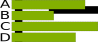
\includegraphics[width=4cm]{img/balkendiagramm.png} &  \includegraphics[width=3cm]{img/kuchendiagramm.png}\\
%%\end{tabular}

\begin{itemize}
\item Säulen- und Kreisdiagramme werden für ordinale und nominale
  Skalen verwendet (und bei quantitativ diskreten Datentypen, wenn es
  nur wenige Ausprägungen sind).
\item Achse: Unverzerrte Skalierung und Beschriftung
\item Legende und Titel
\end{itemize}

\headerUndFooterJedeSeite{}

\begin{tcolorbox}[colback=white]
  \textbf{Absolute und relative Häufigkeit}\\
\begin{tabular}{lcl}

$n$   &$=$& Anzahl Werte\\
$h_i$ &$=$& Absolute Häufigkeit\\
      & & des Merkmals $i$\\
$f_i = \frac{h_i}n$ &$=$& relative Häufigkeit\\
$p_i = f_i\cdot{}100\%$ &$=$& prozentuale Häufigkeit%%\\
%%$\varphi_i = f_i\cdot{}360\degre$ &$=$& Zentriwinkel im\\
%%      & &Kuchendiagramm
  \end{tabular}
\end{tcolorbox}

\headerUndFooterJedeSeite{}

%%\RLP{\forceCB}

\headerUndFooterJedeSeite{}

\subsubsection*{Histogramm}
\headerUndFooterJedeSeite{}
\bbwCenterGraphic{8cm}{img/Histogramm.pdf}

\begin{itemize}
\item Alle Balken sind gleich breit und berühren sich.
\item Die Höhe der Balken wird durch die (absolute / relative) Häufigkeit der entsprechenden
  Werte festgelegt.
\item Die Flächeninhalte der Rechtecke sind proportional
  zu den Häufigkeiten.
\item Die Regeln für die Klassengrenzen müssen festgelegt werden. Zum
  Beispiel Klasse 1: $[160; 170[$
\item Das obige Histogramm ist \textbf{linksschief} und rechtssteil.
\end{itemize}


%Vorgehen
%\begin{enumerate}
%\item Daten in TR eingeben \tiprobutton{data}...
%\item ... und mit \tiprobutton{2nd} \tiprobutton{data_stat-reg-distr} auslesen.
%\item {\color{orange} Median ($\mediantilde{x} = x_{\textrm{MED}}$)},
%und Quartile ({\color{blue}$Q_1$}, {\color{farnFarbe}$Q_3$})einzeichnen
%\item IQR := {\color{farnFarbe}Q3}-{\color{blue}Q1} rechnen
%\item IQR mit 1.5 multiplizieren
%\item {\color{red} untere Ausreisserschwelle\\ uAs} $ = Q_1 -
%1.5\cdot{}\textrm{IQR}$\\ und {\color{red} obere Ausreisserschwelle\\ oAs} $=Q_3 + 1.5\cdot{}\textrm{IQR}$\\ (ausradierbar) fein markieren (gehören nicht zum Boxplot)
%\item Alle Ausreisser mit Ring $\circ$ oder Stern $\star$ einzeichnen.
%\item Whisker (entfernteste Werte innerhalb der Ausreisserschwellen)
%einzeichnen.
%\item Boxdekoration horizontale Linien einzeichnen.
%\end{enumerate}
%\bbwCenterGraphic{8cm}{img/Boxplot.pdf}

\end{multicols}


\headerUndFooterJedeSeite{}
\newpage
\headerUndFooterJedeSeite{}
\subsubsection*{Boxplot}
%%\TRAINER{«Schritte zum Boxplot als Fliesstext
%%  daneben. Ausreisserschwellen {\color{blue}blau} im
%%  Diagramm. Dann im Text auch. Ausreisserschwellen ist ein Begriff von
%%  Frommenwiler, nicht von Marthaler.}%% END TRAINER
Schritte zum Boxplot:\\
Fühler (Whisker) werden auf max. $1.5\cdot\textrm{IQR}$ begrenzt ({\color{blue} Ausreisserschwellen blau})
\ifdefined\versionHECH%%
danach nach \textit{\color{farnFarbe}innen} gehen
\fi%%
: Fühler sind die von der Box
entferntesten Nicht-Ausreisser ({\color{farnFarbe}grün}). Ausreisser
({\color{red} rot}) werden markiert.
\bbwCenterGraphic{18cm}{boxplotRLP.png}

\hrulefill

\begin{multicols}{2}
%%%%%%%%%%%%%%%%%%%%%%%%%%%%%%%%%%%%%%%%%%%%%%%%%%%%%%%%
%%    Kombinatorik / Wahrscheinlichkeit (Stochastik)  %%
%%%%%%%%%%%%%%%%%%%%%%%%%%%%%%%%%%%%%%%%%%%%%%%%%%%%%%%%
\section*{Stochastik}
\headerUndFooterJedeSeite{}

\subsection*{Kombinatorik}

\subsubsection*{Produktregel}

\begin{tabular}{p{5cm}c}
Bsp.: Andrea hat drei verschiedene Hosen und vier verschiedene Pullover.
Es gibt somit $3\cdot{}4$ mögliche Kombinationen.&\raisebox{-3.5cm}{\includegraphics[width=3cm]{img/KombinatorikMultiplikation.pdf}}\end{tabular}


Hat eine zweistufige Situation zunächst $k_1$ Möglichkeiten, gefolgt
von $k_2$ Möglichkeiten, so hat man insgesamt $k_1\cdot{}k_2$
Möglichkeiten. Dies ist auf beliebig viele Stufen verallgemeinerbar.



%%\bbwCenterGraphic{3cm}{img/KombinatorikMultiplikation.pdf}
%%\TRAINER{Ersetze «Ein:e Schüler:in» durch «Andrea»}
%%\forceCB
\subsubsection*{Permutationen (Sitzordnungen)}

Bei $n$ Elementen gibt es $n!$ Permutationen (=Vertauschungen):
                                                                                                                
\begin{tcolorbox}[colback=white]
  \textbf{Fakultät}\\
  $$n! = n\cdot{}(n-1)\cdot{}(n-2)\cdot{}(n-3)\cdot{} ... \cdot{}2\cdot{}1$$
  $$1! = 1\phantom{xxx}0! = 1$$
\end{tcolorbox}



\def\missifarbig{M{\color{farnFarbe}i}{\color{red}ss}{\color{farnFarbe}i}{\color{red}ss}{\color{farnFarbe}i}{\color{cyan}pp}{\color{farnFarbe}i}}

\vspace{3mm}
\textbf{Permutation mit Wiederholung}

oder «\missifarbig»-Formel: Sind bei einer Permutation (Vertauschung) einige Elemente gleich, so reduziert
sich die Anzahl der Möglichkeiten. Wie viele verschiedene Wörter sind mit den Buchstaben des Wortes «\missifarbig» bildbar?
$$N = \frac{11!}{{\color{farnFarbe}4}!\cdot{}{\color{red}4}!\cdot{}{\color{cyan}2}!}$$




\end{multicols}
\newpage
\headerUndFooterJedeSeite{}


\subsection*{Überblick Auswahlprobleme / Anzahl Möglichkeiten $N$ }

$$\textrm{Binomialkoeffizient:} {{\color{blue}n}\choose
{\color{red}k}}
=\frac{{\color{blue}n}!}{({\color{blue}n}-{\color{red}k})!\cdot
{\color{red}k}!}\phantom{etwas Platz lassen} {n\choose 0}= {n\choose
n}= 1$$

\ifisRLP
\bbwCenterGraphic{12cm}{img/KombinatorikRLP.pdf}
\else
\bbwCenterGraphic{13cm}{img/KombinatorikHECH.pdf}
\fi


\hrulefill



\begin{multicols}{2}


\subsection*{Wahrscheinlichkeit}
\subsubsection*{Grundbegriffe}

\textbf{Ergebnismenge} $\Omega$: Menge der möglichen Ergebnisse
(Ausgänge) eines Zufallsversuchs.\\
Beispiel: Die sechs Würfelergebnise
eines Spielwürfels: $\Omega = \left\{\epsdice{1}, \epsdice{2}, \epsdice{3}, \epsdice{4}, \epsdice{5}, \epsdice{6}\right\}$

\textbf{Ereignis} $A$: Eine Teilmenge von $\Omega$. Beispiel: Eine
ungerade Zahl zu werfen: $A  = \left\{\epsdice{1}, \epsdice{3}, \epsdice{5}\right\}$

\textbf{Gegenereignis} $\overline{A} = \Omega \backslash A$ =
\textit{Gegenmenge}

$\overline{A}$ sprich «nicht» $A$.

Es gilt $A \cup \overline{A} = \Omega$

\textbf{Elementarereignis}: Ereignis bestehend aus einem einzigen
Ergebnis aus $\Omega$. Beispiel: $E_1$ = Wirf eine \textbf{Eins}: $E_1
= \left\{\epsdice{1}\right\}$.

%%\forceCB


\subsection*{Laplace-Wahrscheinlichkeit}
Sind alle möglichen Ergebnisse eines Zufallsversuchs gleich
wahrscheinlich (fairer Würfel), so ist die Wahrscheinlichkeit $P(E)$ für das Ereignis
$E$ wie folgt zu berechnen:

$$P(E) = \frac{\textrm{Anzahl Ergebnisse in
}E}{\textrm{Anzahl Ergebnisse in }\Omega}$$%%
%%
\forceCB%%
\subsubsection*{Baumdiagramme}
Bsp.: Zwei Mal eine \textit{unfaire} Münze werfen
\bbwCenterGraphic{75mm}{img/WahrscheinlichkeitBaumdiagramm.pdf}

Wahrscheinlichkeiten {\color{farnFarbe}entlang} eines Pfades werden {\color{farnFarbe}multipliziert}:
$$P(KK) = 0.6\cdot0.6=0.36$$

Wahrscheinlichkeiten {\color{red}verschiedener} Pfade werden
{\color{red}addiert}:

\begin{tabular}{rcl}
${\color{red}P}({\color{farnFarbe}KK} \textrm{\color{red} oder } {\color{blue}ZZ})$ &=&
  $P({\color{farnFarbe}KK}) {\color{red}+} P({\color{blue}ZZ})$\\
  &=&${\color{farnFarbe}0.6\cdot0.6} {\color{red}+} {\color{blue}0.4\cdot0.4}$
\end{tabular}

\forceCB{}

\subsection*{Binomialverteilung}
\subsubsection*{Bernoulli}
\headerUndFooterJedeSeite{}

Ein Experiment wird $n$ mal ausgeführt.

Jede Ausführung hat die selbe Trefferwahrscheinlichkeit $p$.

Die Wahrscheinlichkeit für \textbf{genau} $x$ Treffer ist


\begin{tcolorbox}[colback=white]
$$P(X=x) = {n \choose x}\cdot{}p^x\cdot{}(1-p)^{n-x}$$
Taschenrechner:  \textbf{\texttt{binomialpdf}}
\end{tcolorbox}%%

Beispiel: Ein Spieler trifft mit 35\% Wahrscheinlichkeit
($p=0.35$). Wie gross ist die Wahrscheinlichkeit, dass er mit 20 Würfen
($n=20$) \textbf{genau} vier Mal ($x=4$) trifft?

Lösung: \texttt{binomialpdf} $\Longrightarrow 7.38\%$


\subsubsection*{Kumulierte Binomialverteilung}

\begin{tcolorbox}[colback=white]
$$P(X\le x) = \sum_{j=0}^{x}{n \choose j}\cdot{}p^j\cdot{}(1-p)^{n-j}$$
$x$ = \textbf{maximal} gewünschte Anzahl Treffer\\
$n$ = Anzahl Ausführungen\\
$p$ = Trefferwahrscheinlichkeit\\
Taschenrechner: \textbf{\texttt{binomialcdf}}
\end{tcolorbox}

%%\forceCB{}

\subsection*{Lottomodell}
(Hypergeometrische Verteilung)

\ifisRLP
\begin{tcolorbox}[colback=white]
Gegeben $n$ Kugeln in einer Urne. Herausgezogen werden $k$:
\begin{itemize}
\item $t =$ Anzahl der \textit{guten} Kugeln
\end{itemize}
Wahrscheinlichkeit \textbf{genau} $x$ \textit{gute} Kugeln zu ziehen:

$$P(X=x) = \frac{ {t \choose x} \cdot {n-t  \choose k-x} }{{n \choose k}}$$
\end{tcolorbox}
\else
\begin{tcolorbox}[colback=white]
Gegeben $N+T$ Kugeln in einer Urne. Herausgezogen werden $n+t$:
\begin{itemize}
\item $T$ Anzahl aller Treffer
\item $N$ Anzahl aller Nieten
\item $t$ gewünschte Treffer
\item $n$ «gewünschte» Nieten
\end{itemize}
Wahrscheinlichkeit \textbf{genau} $t$ Treffer zu ziehen:

$$P_{N,T,n}(X=t) = \frac{ {T \choose t} \cdot {N  \choose n} }{{T+N \choose t+n}}$$
\end{tcolorbox}
\fi%% END RLP


\subsection*{Elementare Wahrscheinlichkeit}
Ereignisse sind voneinander \textbf{unabhängig}, wenn sie keine
gleichen Ergebnisse aufweisen.
$$A \textrm{ unabhängig von } B \Leftrightarrow A\cap B=\{\}$$

Für voneinander \textbf{unabhängige} Ergebnisse 
gilt:

$$P(A\textrm{ «oder» }B) = P(A\cup B) = P(A) + P(B)$$
\headerUndFooterJedeSeite{}

%%\forceCB
%%\headerUndFooterJedeSeite{}

\subsubsection*{Gegenwahrscheinlichkeit}
Die Wahrscheinlichkeit des \textbf{Gegenereignisses} von $E$ ist
$$P(\overline{E}) = 1- P(E)$$

Bei Aufgaben wie «... mindestens eins ...» ist das Arbeiten mit der
Gegenwahrscheinlichkeit häufig einfacher.

\textbf{Beispiel}: Das Gegenteil von «Spieler trifft minimal vier Mal»
ist «Spieler trifft maximal drei Mal»:

$$P(X \ge 4) = 1 - P(X < 4) = 1-P(X\le 3)$$

Gegenereignis von «minimal 4 Mal» = «maximal 3 Mal».

\headerUndFooterJedeSeite{}

\forceCB{}
\subsection*{Zufallsgrössen, Zufallsvariable $\mathbf{X}$}
\headerUndFooterJedeSeite{}

(mit endlich vielen Werten $x_i$)

\subsubsection*{Zufallsvariable $\mathbf{X}$}

Eine Zufallsvariable ordnet jedem Element von $\Omega$, d.\,h. jedem
Ergebnis, eine Zahl zu.

Beispiel: 3 Münzen gleichzeitig werfen K = „Kopf“, Z = „Zahl“.
Zufallsgrösse $X$ sei \zB die Anzahl „Köpfe“.
Dem Ergebnis (KKZ) wird somit die Zahl 2 zugeordnet.

\subsubsection*{Erwartungswert $\mu$ derZufallsgrösse $\mathbf{X}$}
$\mu$ gibt den auf lange Sicht zu erwartenden Mittelwert der
Zufallsgrösse an:

\begin{tabular}{cp{5cm}}
\hline\\
\raisebox{-4mm}{\fbox{$\mu=\sum\limits_{i=1}^n x_i\cdot{}p_i$}} & $x_i$ = $i$-ter Wert der
Zufallsgrösse. $p_i$ = Wahrscheinlichkeit  $P(X=x_i)$\\
 \hline
 \end{tabular}

%%\forceCB{}

\subsection*{Vierfeldtafeln}
Vierfeld-Tafeln=Kontingenztafeln mit 4 Feldern.

Man hat zwei Merkmale, A und B. Jedes Merkmal kann nur zwei Werte
annehmen (+ / -). Dies ergibt vier Möglichkeiten. Die Vierfeldtafel
enthält die absoluten oder die relativen Häufigkeiten der vier
Kombinationen der Merkmalswerte.

Zudem werden noch die Randsummen notiert.


\begin{tabular}{c|c|c|c}
           & gesund (G)& krank (K)& $\Sigma$ \\\hline
Frauen (F) &        30 &       40 &       70 \\\hline
Männer (M) &        25 &       35 &       60 \\\hline
$\Sigma$   &        55 &       75 &      130 \\\hline
 \end{tabular}

%%\bbwCenterGraphic{8cm}{img/kontingenztafel.png}


\subsection*{Bedingte Wahrscheinlichkeit}

%\begin{tcolorbox}[colback=white]
%%  \textbf{Bedingte Wahrscheinlichkeit}\\
%Mit
%$$P(A|B)$$
%Wird die Wahrscheinlichkeit von $A$ angegeben, unter der Bedingung,
%dass das Ereignis $B$ bereits eingetroffen ist.
%\end{tcolorbox}
%\mmPap{10.4}%

Mit den Zahlen aus obigem Beispiel gilt:

\textbf{Normale Wahrscheinlichkeit}\\
«Wie gross ist hier die Wahrscheinlichkeit, gesund (G) zu sein?»
$$P(G) = \frac{\textrm{Anzahl Gesunde}}{\textrm{Alle}} =  \frac{55}{130}$$

\textbf{Wahrscheinlichkeit der Schnittmenge}\\
«Wie gross ist hier die Wahrscheinlichkeit, eine gesunde Frau anzutreffen treffen?»
$$P(G\cap F) = \frac{\textrm{\ Anzahl gesunde Frauen}}{\textrm{Alle}}= \frac{30}{130}$$

\textbf{Bedingte Wahrscheinlichkeit}\\
«Wie gross ist die Wahrscheinlichkeit, unter den Gesunden eine Frau anzutreffen?»
$$P(F | G) = \frac{\textrm{Anzahl gesunde Frauen}}{\textrm{Anzahl Gesunde}} =  \frac{30}{55}$$
«Wie gross ist die Wahrscheinlichkeit, unter den Frauen eine gesunde Person zu treffen?»
$$P(G | F) = \frac{\textrm{Anzahl gesunde Frauen}}{\textrm{Anzahl Frauen}}=  \frac{30}{70}$$

\end{multicols}


%% Leerseiten für Notizen
\newpage
\headerUndFooterJedeSeite{}

%%%%%%%%%%%%%%%%%%%%%%%%%%%%%%%%%%%%%%%%%%%%%%%%%%%%%%%%
%%               Taschenrechner                       %%
%%%%%%%%%%%%%%%%%%%%%%%%%%%%%%%%%%%%%%%%%%%%%%%%%%%%%%%%
\section*{Taschenrechner}

\begin{tabular}{cc}


\raisebox{-45mm}{\includegraphics[width=45mm]{img/tiprobuttonimages/ti30.png}}
&

\begin{tabular}{c|c|p{80mm}}\hline
\tiprobutton{math}         &Summe             & Summenzeichen $\Sigma$ (\tiprobutton{5})\\
                           &Faktorzerlegung   & Faktorzerlegung (\tiprobutton{4}\texttt{Pfactor})\\
                           & ggT, kgV         & gcd = ggT
(\tiprobutton{3}), lcm = kgV (\tiprobutton{2})\\\hline
                           &                  & Bestimmung statistischer Werte:\\
\tiprobutton{data}         & data             & Daten eingeben\\
                           &\texttt{stat-reg} & 1-VAR STATS anwählen
und \texttt{calc} drücken für Standardabweichung, Q1, Q3, Median, Min,
Max, Mittelwert etc.\\
                           &\texttt{distr}    & Bernoulliformel $\rightarrow$ 4: Binomial\textbf{p}df\\
                           &                  & Kumuliert $\rightarrow$ 5: Binomial\textbf{c}df\\\hline
\tiprobutton{cos_poly-solv}&\texttt{poly-solv}&  Quadratische Gleichungen in Grundform $ax^2+bx+c=0$\\
                           &                  &  (Auch für Zweiklammeransatz)\\\hline
\tiprobutton{tan_sys-solv} &\texttt{sys-solv} &  Lineare Gleichungssysteme\\\hline
\tiprobutton{sin_num-solv} &\texttt{num-solv} &  Gleichungen ($7^x=3^{2x+1}$) mit Zahlen nach $x$ auf\/lösen (hier $x\approx{}-4.37$).\\\hline
\tiprobutton{table}        & table            &  Wertetabelle für diverse Funktionen: Lineare Fkt., Potenzfkt., Exponentialfkt.\\\hline
\tiprobutton{ncrnpr}       &Kombinatorik      &  Fakultät: {\color{red}\textbf{!}}\\
                           &                  &  Kombination $n \choose k$ tippe $n$ nCr $k$\\
                           &                  &  Permutation $\frac{n!}{(n-k)!}$ tippe $n$ nPr $k$\\\hline
\tiprobutton{ln_log}       &  Logarithmen     &  log = Zehnerlogarithmus ($\lg$)\\
                           &                  &  ln  = Log. zur Basis $e$\\
                           &                  &  3x drücken = log zu beliebiger Basis\\\hline
\tiprobutton{sto_recall}   & Werte speichern  &  Erst \texttt{sto} drücken, danach können die Variablen gespeichert werden (\tiprobutton{xyzabcd}). \\\hline
\tiprobutton{xyzabcd}      &                  & Benutzen und Auslesen der Variablen.\\\hline
\tiprobutton{approx}       & Resultat-Anzeige  & $\sqrt{50}$ = $5\sqrt{2} \approx 7.0711$
\end{tabular}
\end{tabular}

\TRAINER{{\small Generelle Fragen:\\
Fehlen Lernziele? Sind Lernziele zu viel?\\
Sind Beispiele zu viel/zu wenig?\\
Hat es genügend Platz für die SuS (Schülerinnen und Schüler) für weitere Notizen/Beispiele/Rezepte/Vorgehen?\\
Ganz am Schluss:

* Rechtschreibeprogramm
* Zeilenumbrüche und Einzüge (0pt bei Aufzählungen und Nummerierungen)
* Absatz-Umbrüche / Seitenumbrüche
}}
\headerUndFooterJedeSeite{}

%
\noTRAINER{\vspace{15mm}}%
%
%%\noTRAINER{\mmPapier{4}}%
%
\headerUndFooterJedeSeite{}
\newpage
\headerUndFooterJedeSeite{}

%%%%%%%%%%%%%%%%%%%%%%%%%%%%%%%%%%%%%%%%%%%%%%
%%           Notizen                        %%
%%%%%%%%%%%%%%%%%%%%%%%%%%%%%%%%%%%%%%%%%%%%%%

Eigene Notizen\\

\noTRAINER{\mmPapier{22}}%
\TRAINER{\mmPapier{20}}%
%
\vspace{5mm}

Fehler gefunden? \texttt{philipp.freimann@bbw.ch / christian.hersberger@bbw.ch}

\tiny{\versionsnummerFoSa}

\TRAINER{
{\footnotesize Quelltext dieser Formelsammlung:\\
\texttt{https://github.com/pheek/bbwMathe/tree/main/arbeitsblaetter/formelsammlung}}

{\footnotesize Version \versionsnummerFoSa{}}
}%% END TRAINER


\end{document}
